\begin{center}
  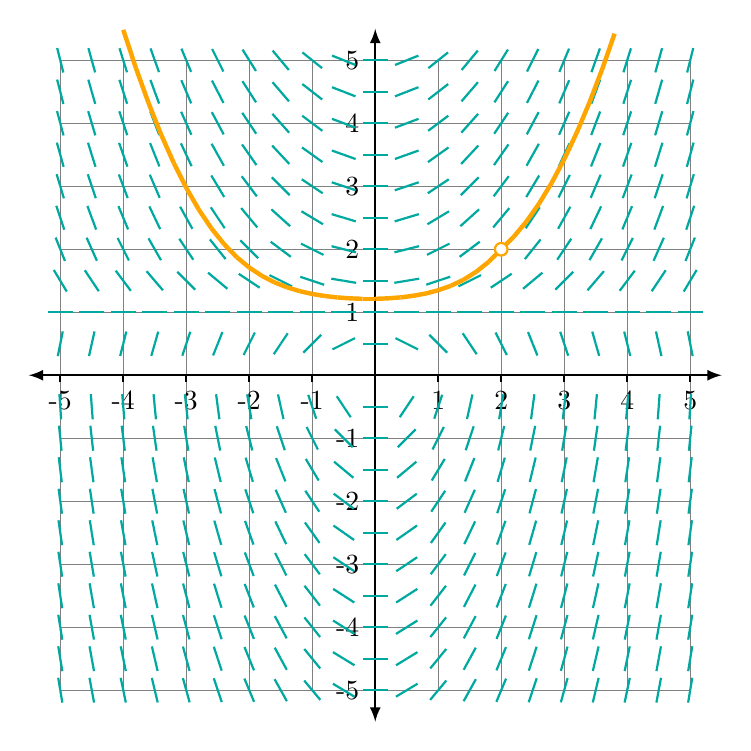
\begin{tikzpicture}
      \begin{scope}[scale=0.8]
          \def\dx{0.5}; % x-spacing for ticks
          \def\dy{0.5}; % y-spacing for ticks
          \def\sx{-5};  % lower bound for x values
          \def\sy{-5};  % lower bound for y values
          \def\ex{5};   % upper bound for x values
          \def\ey{5};   % upper bound for y values
          \def\l{0.2};  % length of HALF of a segment
          
          % draw grid
          \draw[Gray, thin] (-5,-5) grid (5,5);
          \draw[thick,latex-latex] (-5.5,0) -- (5.5,0);
          \draw[thick,latex-latex] (0,-5.5) -- (0,5.5);
          
          \foreach \i in {-5,...,-1,1,2,...,5} {
            \draw[thick] (\i,0)--(\i,-0.1);
            \node[below] at (\i,-0.1) {\i};
            \draw[thick] (0,\i)--(-0.1,\i);
            \node[left] at (-0.1,\i) {\i};
          }
          
          % draw slope ticks:
          \foreach \x  in {-5,-4.5,...,5} {
            \foreach \y  in {-5,-4.5,...,-0.5,0.5,1,...,5} {
              \pgfmathsetmacro{\m}{\x-\x/\y};
              \pgfmathsetmacro{\k}{\l/sqrt(1+\m*\m)};
              \pgfmathsetmacro{\h}{\k*\m};
              \draw[ thick, Emerald] (\x,\y) -- (\x+\k,\y+\h);
              \draw[ thick, Emerald] (\x,\y) -- (\x-\k,\y-\h);
            }
          }
          
          % Euler's method
          \pgfmathsetmacro{\lasty}{2};
          \foreach \x in {2.2,2.4,...,3.8} {
            \pgfmathsetmacro{\thisx}{\x};
            \pgfmathsetmacro{\lastx}{\x-0.2};
            \pgfmathsetmacro{\f}{\lastx-\lastx/\lasty};
            \pgfmathsetmacro{\thisy}{\lasty + 0.2*\f};
            \draw[ultra thick, Orange] (\lastx,\lasty) -- (\thisx,\thisy);
            \global\let\lasty = \thisy;
          }
          \pgfmathsetmacro{\lasty}{2};
          \foreach \x in {1.8,1.6,...,-4} {
            \pgfmathsetmacro{\thisx}{\x};
            \pgfmathsetmacro{\lastx}{\x+0.2};
            \pgfmathsetmacro{\f}{\lastx-\lastx/\lasty};
            \pgfmathsetmacro{\thisy}{\lasty - 0.2*\f};
            \draw[ultra thick, Orange] (\lastx,\lasty) -- (\thisx,\thisy);
            \global\let\lasty = \thisy;
          }
          \draw[Orange,fill=white,thick] (2,2) circle (0.1);
          \end{scope}
          
  \end{tikzpicture}
\end{center}